\chapter{HASIL DAN PEMBAHASAN}
\label{chap:pengujiananalisis}

% Ubah bagian-bagian berikut dengan isi dari pengujian dan analisis

Pada penelitian ini akan dipaparkan hasil dan pembahasan dari proses-proses yang telah dilakukan pada
bab metodologi. Hasil pembahasan yang ada pada bab ini diharapkan agar dapat ditarik suatu kesimpulan
dari pelaksanaan tugas akhir yang telah dilakukan.

\section{Hasil Pengumpulan Data}
\label{sec:skenariopengujian}

Video yang digunakan sebagai masukan dari model yang dibuat, diambil dari dataset UTA-RLDD. Banyak video yang perlu disaring
pada dataset ini guna menghasilkan data yang cukup baik. Video dengan fps yang mendekati 30 fps saja yang dapat digunakan sebagai
data masukan model. Didapatkan sebanyak 42 video pada setiap kelas seperti gambar \ref{tb:JumlahVideo} sehingga jumlah video
yang dapat diekstraksi datanya berjumlah 126 video. Video yang ada pada dataset ini terbagi menjadi 3 kelas berbeda yaitu
kelas 1 (Waspada), kelas 2 (Kewaspadaan Rendah), serta kelas 3 (Mengantuk). Subjek pada video yang diambil terdiri dari pria
dan wanita yang berasal dari berbagai etnis serta sejumlah subjek yang ada pada video memakai kacamata serta memiliki bulu
yang lebat di wajah. Berikut merupakan gambar sebaran jumlah video berdasarkan masing-masing kelas:

\begin{longtable}{|c|c|}
  \caption{Sebaran Video Tiap Kelas}
  \label{tb:JumlahVideo}                 \\
  \hline
  \rowcolor[HTML]{C0C0C0}
  \textbf{Kelas} & \textbf{Jumlah Video} \\
  \hline
  1              & 42                    \\
  2              & 42                    \\
  3              & 42                    \\
  \hline
\end{longtable}

\section{Hasil Ekstraksi Fitur}
Ekstraksi fitur dilakukan secara lokal dengan bantuan IDE PyCharm edisi 2021.3.3 menghasilkan
koordinat setiap titik pada mata maupun mulut berupa sumbu (x, y). Titik-titik koordinat tersebut nantinya
akan digunakan untuk melakukan perhitungan sesuai dengan rumus \ref{eq:EAR} untuk menghasilkan nilai EAR
serta rumus \ref{eq:MAR} untuk menghasikan nilai MAR. Berikut merupakan gambaran data-data yang didapat
setelah melakukan ekstraksi fitur:

\begin{longtable}{|c|c|c|c|}
  \caption{Deskripsi Data Hasil Ekstraksi Fitur}
  \label{tb:DeskripsiData}                                                                          \\
  \hline
  \rowcolor[HTML]{C0C0C0}
  \textbf{No} & \textbf{Nama Kolom} & \textbf{Tipe Data} & \textbf{Deskripsi}                       \\
  \hline
  1           & frame               & \textit{integer}   & Jumlah Frame                             \\
  2           & timestamp\_x        & \textit{float}     & Waktu (detik)                            \\
  3           & xl0\_x              & \textit{float}     & Titik x pada koordinat 36 Landmark Wajah \\
  4           & yl0\_x              & \textit{float}     & Titik y pada koordinat 36 Landmark Wajah \\
  5           & xl1\_x              & \textit{float}     & Titik x pada koordinat 37 Landmark Wajah \\
  6           & yl1\_x              & \textit{float}     & Titik y pada koordinat 37 Landmark Wajah \\
  7           & xl2\_x              & \textit{float}     & Titik x pada koordinat 38 Landmark Wajah \\
  8           & yl2\_x              & \textit{float}     & Titik y pada koordinat 38 Landmark Wajah \\
  9           & xl3\_x              & \textit{float}     & Titik x pada koordinat 39 Landmark Wajah \\
  10          & yl3\_x              & \textit{float}     & Titik y pada koordinat 39 Landmark Wajah \\
  11          & xl4\_x              & \textit{float}     & Titik x pada koordinat 40 Landmark Wajah \\
  12          & yl4\_x              & \textit{float}     & Titik y pada koordinat 40 Landmark Wajah \\
  13          & xl5\_x              & \textit{float}     & Titik x pada koordinat 41 Landmark Wajah \\
  14          & yl5\_x              & \textit{float}     & Titik y pada koordinat 41 Landmark Wajah \\
  15          & xr0\_x              & \textit{float}     & Titik x pada koordinat 42 Landmark Wajah \\
  16          & yr0\_x              & \textit{float}     & Titik y pada koordinat 42 Landmark Wajah \\
  17          & xr1\_x              & \textit{float}     & Titik x pada koordinat 43 Landmark Wajah \\
  18          & yr1\_x              & \textit{float}     & Titik y pada koordinat 43 Landmark Wajah \\
  19          & xr2\_x              & \textit{float}     & Titik x pada koordinat 44 Landmark Wajah \\
  20          & yr2\_x              & \textit{float}     & Titik y pada koordinat 44 Landmark Wajah \\
  21          & xr3\_x              & \textit{float}     & Titik x pada koordinat 45 Landmark Wajah \\
  22          & yr3\_x              & \textit{float}     & Titik y pada koordinat 45 Landmark Wajah \\
  23          & xr4\_x              & \textit{float}     & Titik x pada koordinat 46 Landmark Wajah \\
  24          & yr4\_x              & \textit{float}     & Titik y pada koordinat 46 Landmark Wajah \\
  25          & xr5\_x              & \textit{float}     & Titik x pada koordinat 47 Landmark Wajah \\
  26          & yr5\_x              & \textit{float}     & Titik y pada koordinat 47 Landmark Wajah \\
  27          & ear\_x              & \textit{float}     & Nilai Kalkulasi EAR                      \\
  28          & x0\_x               & \textit{float}     & Titik x pada koordinat 60 Landmark Wajah \\
  29          & y0\_x               & \textit{float}     & Titik y pada koordinat 60 Landmark Wajah \\
  30          & x1\_x               & \textit{float}     & Titik x pada koordinat 61 Landmark Wajah \\
  31          & y1\_x               & \textit{float}     & Titik y pada koordinat 61 Landmark Wajah \\
  32          & x2\_x               & \textit{float}     & Titik x pada koordinat 62 Landmark Wajah \\
  33          & y2\_x               & \textit{float}     & Titik y pada koordinat 62 Landmark Wajah \\
  34          & x3\_x               & \textit{float}     & Titik x pada koordinat 63 Landmark Wajah \\
  35          & y3\_x               & \textit{float}     & Titik y pada koordinat 63 Landmark Wajah \\
  36          & x4\_x               & \textit{float}     & Titik x pada koordinat 64 Landmark Wajah \\
  37          & y4\_x               & \textit{float}     & Titik y pada koordinat 64 Landmark Wajah \\
  38          & x5\_x               & \textit{float}     & Titik x pada koordinat 65 Landmark Wajah \\
  39          & y5\_x               & \textit{float}     & Titik y pada koordinat 65 Landmark Wajah \\
  40          & x6\_x               & \textit{float}     & Titik x pada koordinat 66 Landmark Wajah \\
  41          & y6\_x               & \textit{float}     & Titik y pada koordinat 66 Landmark Wajah \\
  42          & x7\_x               & \textit{float}     & Titik x pada koordinat 67 Landmark Wajah \\
  43          & y7\_x               & \textit{float}     & Titik y pada koordinat 67 Landmark Wajah \\
  44          & mar\_x              & \textit{float}     & Nilai Kalkulasi MAR                      \\
  \hline
\end{longtable}

\section{Hasil Preprocessing}

Preprocessing data dilakukan untuk menyiapkan data pelatihan model sehingga dapat menghasilkan
model klasifikasi yang baik. Berikut hasil implementasikan praproses data pada pengembangan penelitian
diantaranya melakukan ekstraksi fitur, mengatasi data/frame kosong, melakukan penyetaraan jumlah data
dan labeling, melakukan normalisasi data, serta melakukan penyesuaian bentuk data.

\subsection{Hasil Interpolasi Data}
Video yang telah terpilih tidak selalu memiliki data yang lengkap pada tiap frame. Terdapat data yang
bernilai NaN dikarenakan koordinat landmark wajahnya tidak terdeteksi. Oleh karena itu digunakan interpolasi
linear untuk mengisi data yang nilainya NaN sehingga titik-titik koordinat yang dibutuhkan untuk menghitung
nilai EAR maupun MAR menjadi lengkap dan bisa mendapatkan nilai dari EAR maupun MAR itu sendiri. Berikut
merupakan contoh tabel data yang memiliki nilai NaN di dalamnya sebelum maupun setelah dilakukannya
interpolasi:

\begin{longtable}{|c|c|c|c|}
  \caption{Data Kosong Sebelum Interpolasi}
  \label{tb:NaNdata}                                                       \\
  \hline
  \rowcolor[HTML]{C0C0C0}
  \textbf{timestamp\_x} & \textbf{xl0\_x} & \textbf{...} & \textbf{mar\_x} \\
  \hline
  10.329                & 78              & ...          & 0.1197736075    \\
  10.362                & 78              & ...          & 0.1427218439    \\
  10.395                & NaN             & ...          & NaN             \\
  10.428                & NaN             & ...          & NaN             \\
  10.461                & 77              & ...          & 0.1290500622    \\
  10.494                & 77              & ...          & 0.1433720878    \\
  10.527                & 78              & ...          & 0.1215658232    \\
  \hline
\end{longtable}

\begin{longtable}{|c|c|c|c|}
  \caption{Data Kosong Setelah Interpolasi}
  \label{tb:noNaNdata}                                                     \\
  \hline
  \rowcolor[HTML]{C0C0C0}
  \textbf{timestamp\_x} & \textbf{xl0\_x} & \textbf{...} & \textbf{mar\_x} \\
  \hline
  10.329                & 78              & ...          & 0.1197736075    \\
  10.362                & 78              & ...          & 0.1427218439    \\
  10.395                & 78              & ...          & 0.05930266631   \\
  10.428                & 77              & ...          & 0.05930266631   \\
  10.461                & 77              & ...          & 0.1290500622    \\
  10.494                & 77              & ...          & 0.1433720878    \\
  10.527                & 78              & ...          & 0.1215658232    \\
  \hline
\end{longtable}


\subsection{Hasil Penyetaraan Data dan Labeling}
Panjang data yang didapatkan pada setiap video tidaklah sama seperti pada tabel \ref{tb:JumlahData}, oleh karena itu
perlu dilakukan penyetaraan panjang data pada tiap video sehingga dapat menjadi
inputan untuk model klasifikasi. Pada tahap ini hanya kolom ear\_x dan mar\_x
saja yang digunakan. Panjang data yang dibutuhkan adalah 16200 data tiap video.
Setelah jumlah data diseragamkan, maka data-data tersebut akan diberi label tiap
frame sesuai dengan label yang telah ditentukan oleh dataset UTA-RLDD. Berikut
merupakan tabel rincian jumlah data yang didapat yang ada pada setiap video:

\begin{longtable}{|c|c|c|c|c|c|c|c|c|}
  \caption{Jumlah Data Pada Tiap Video}
  \label{tb:JumlahData}                                                                                                                      \\
  \hline
  \rowcolor[HTML]{C0C0C0}
  \textbf{No} & \textbf{Video} & \textbf{Data} & \textbf{No} & \textbf{Video} & \textbf{Data} & \textbf{No} & \textbf{Video} & \textbf{Data} \\
  \hline
  1           & 13-1.csv       & 18234         & 43          & 10-2.csv       & 18620         & 85          & 10-3.csv       & 18866         \\
  2           & 35-1.csv       & 18027         & 44          & 13-2.csv       & 20477         & 86          & 13-3.csv       & 18486         \\
  3           & 59-1.csv       & 18089         & 45          & 59-2.csv       & 18169         & 87          & 34-3.csv       & 18388         \\
  4           & 7-1.csv        & 18016         & 46          & 19-2.csv       & 18035         & 88          & 35-3.csv       & 18340         \\
  5           & 21-1.csv       & 18151         & 47          & 21-2.csv       & 18031         & 89          & 59-3.csv       & 18095         \\
  6           & 19-1.csv       & 18029         & 48          & 9-2.csv        & 18367         & 90          & 7-3.csv        & 17939         \\
  7           & 9-1.csv        & 18172         & 49          & 34-2.csv       & 20693         & 91          & 20-3.csv       & 21437         \\
  8           & 60-1.csv       & 18054         & 50          & 60-2.csv       & 17533         & 92          & 19-3.csv       & 18064         \\
  9           & 42-1.csv       & 18021         & 51          & 35-2.csv       & 18022         & 93          & 21-3.csv       & 18055         \\
  10          & 5-1.csv        & 18410         & 52          & 56-2.csv       & 18354         & 94          & 9-3.csv        & 19816         \\
  11          & 8-1.csv        & 18158         & 53          & 42-2.csv       & 18122         & 95          & 60-3.csv       & 18581         \\
  12          & 10-1.csv       & 16417         & 54          & 40-2.csv       & 18036         & 96          & 5-3.csv        & 18050         \\
  13          & 56-1.csv       & 18355         & 55          & 36-2.csv       & 18792         & 97          & 8-3.csv        & 17989         \\
  14          & 14-1.csv       & 18386         & 56          & 5-2.csv        & 18062         & 98          & 56-3.csv       & 19417         \\
  15          & 15-1.csv       & 19301         & 57          & 7-2.csv        & 17886         & 99          & 14-3.csv       & 18692         \\
  16          & 22-1.csv       & 18221         & 58          & 14-2.csv       & 19742         & 100         & 15-3.csv       & 18483         \\
  17          & 1-1.csv        & 18055         & 59          & 15-2.csv       & 18541         & 101         & 22-3.csv       & 18316         \\
  18          & 2-1.csv        & 18263         & 60          & 22-2.csv       & 18266         & 102         & 1-3.csv        & 18012         \\
  19          & 17-1.csv       & 18121         & 61          & 1-2.csv        & 18033         & 103         & 2-3.csv        & 18124         \\
  20          & 12-1.csv       & 16919         & 62          & 2-2.csv        & 18106         & 104         & 3-3.csv        & 18480         \\
  21          & 23-1.csv       & 17567         & 63          & 8-2.csv        & 18048         & 105         & 17-3.csv       & 18212         \\
  22          & 20-1.csv       & 19122         & 64          & 3-2.csv        & 18514         & 106         & 23-3.csv       & 18187         \\
  23          & 25-1.csv       & 17992         & 65          & 17-2.csv       & 18245         & 107         & 25-3.csv       & 17987         \\
  24          & 26-1.csv       & 18489         & 66          & 12-2.csv       & 18838         & 108         & 26-3.csv       & 20849         \\
  25          & 27-1.csv       & 19724         & 67          & 20-2.csv       & 17957         & 109         & 27-3.csv       & 18627         \\
  26          & 30-1.csv       & 20439         & 68          & 23-2.csv       & 17286         & 110         & 30-3.csv       & 18251         \\
  27          & 36-1.csv       & 18694         & 69          & 25-2.csv       & 18016         & 111         & 36-3.csv       & 18728         \\
  28          & 37-1.csv       & 20483         & 70          & 26-2.csv       & 26445         & 112         & 37-3.csv       & 20396         \\
  29          & 38-1.csv       & 18056         & 71          & 27-2.csv       & 18774         & 113         & 39-3.csv       & 18158         \\
  30          & 39-1.csv       & 19376         & 72          & 30-2.csv       & 20846         & 114         & 40-3.csv       & 18029         \\
  31          & 40-1.csv       & 18060         & 73          & 37-2.csv       & 18551         & 115         & 41-3.csv       & 25166         \\
  32          & 41-1.csv       & 18839         & 74          & 38-2.csv       & 18097         & 116         & 42-3.csv       & 18030         \\
  33          & 43-1.csv       & 35818         & 75          & 39-2.csv       & 18173         & 117         & 43-3.csv       & 34975         \\
  34          & 48-1.csv       & 18913         & 76          & 43-2.csv       & 35936         & 118         & 46-3.csv       & 17773         \\
  35          & 47-1.csv       & 18027         & 77          & 48-2.csv       & 18183         & 119         & 47-3.csv       & 18340         \\
  36          & 58-1.csv       & 18054         & 78          & 47-2.csv       & 18022         & 120         & 54-3.csv       & 18944         \\
  37          & 54-1.csv       & 19107         & 79          & 58-2.csv       & 18302         & 121         & 58-3.csv       & 18244         \\
  38          & 49-1.csv       & 18191         & 80          & 49-2.csv       & 17917         & 122         & 50-3.csv       & 20013         \\
  39          & 50-1.csv       & 18174         & 81          & 50-2.csv       & 21683         & 123         & 51-3.csv       & 18494         \\
  40          & 51-1.csv       & 18182         & 82          & 51-2.csv       & 18364         & 124         & 52-3.csv       & 18077         \\
  41          & 52-1.csv       & 18044         & 83          & 52-2.csv       & 18062         & 125         & 38-3.csv       & 18074         \\
  42          & 57-1.csv       & 18938         & 84          & 57-2.csv       & 18221         & 126         & 57-3.csv       & 18368         \\
  \hline
\end{longtable}

\subsection{Hasil Normalisasi Data}
Normalisasi data Z-score dilakukan dengan menggunakan fungsi Standard Scaler pada library sklearn. Rumus yang digunakan untuk mencari
Z-score dari setiap data adalah rumus \ref{eq:StandardScaler}. Cara kerjanya sendiri yaitu data akan dikurangi dengan nilai rata-rata
dari keseluruhan data kemudian dibagi oleh standard deviasi dari keseluruhan data. Normalisasi ini menyebabkan semua fitur
memiliki skala yang serupa, sehingga memudahkan perbandingan dan interpretasi data. Berikut merupakan data sebelum dan sesudah
dinormalisasi:

\begin{longtable}{|c|c|c|c|}
  \caption{Data Sebelum Normalisasi}
  \label{tb:NaNdata}                                             \\
  \hline
  \rowcolor[HTML]{C0C0C0}
  \textbf{} & \textbf{ear\_x} & \textbf{mar\_x} & \textbf{label} \\
  \hline
  0         & 0.296401        & 0.067902        & 1              \\
  1         & 0.309457        & 0.054692        & 1              \\
  2         & 0.289860        & 0.068918        & 1              \\
  3         & 0.289045        & 0.044270        & 1              \\
  4         & 0.299951        & 0.046012        & 1              \\
  ...       & ...             & ...             & ...            \\
  2041199   & 0.259205        & 0.176349        & 3              \\
  \hline
\end{longtable}

\begin{longtable}{|c|c|c|c|}
  \caption{Data Setelah Normalisasi}
  \label{tb:NaNdata}                                             \\
  \hline
  \rowcolor[HTML]{C0C0C0}
  \textbf{} & \textbf{ear\_x} & \textbf{mar\_x} & \textbf{label} \\
  \hline
  0         & 0.166568        & 0.544814        & 1              \\
  1         & 0.399185        & 0.270716        & 1              \\
  2         & 0.050017        & 0.565894        & 1              \\
  3         & 0.035485        & 0.054473        & 1              \\
  4         & 0.229822        & 0.090614        & 1              \\
  ...       & ...             & ...             & ...            \\
  2041199   & -0.496194       & 2.794994        & 3              \\
  \hline
\end{longtable}

Setelah data dinormlisasi, data kemudian dibagi menjadi data untuk train sebanyak 101 video
dan data test atau val sebanyak 25 video. Data train kemudian dilakukan augmentasi hingga
menjadi 353 video untuk menghindari overfitting pada model.

\subsection{Hasil Sliding Window}

Bentuk data masukan yang dimiliki adalah 2 dimensi dimana bentuk data training yaitu (5718600, 2) dan
bentuk data test/validasi yaitu (405000, 2) sedangkan yang dibutuhkan pada model IndRNN berjumlah 3 dimensi sehingga sliding window
diperlukan agar bentuk data trainingnya menjadi (353, 16200, 2) dan bentuk data test/validasi (25, 16200, 2). Bentuk data tersebut dapat
dijelaskan menjadi angka pertama merupakan jumlah video, 16200 merupakan jumlah langkah waktu / frame dalam satu video, serta 2
merupakan jumlah fitur yang digunakan yaitu EAR dan MAR.

\section{Hasil Training Data}
\subsection{Independent Recurrent Neural Network}
Berikut merupakan gambar loss dan akurasi dari data training yang tidak teraugmentasi dan
data validasi yang terbaik:

\begin{figure} [H] \centering
  % Nama dari file gambar yang diinputkan
  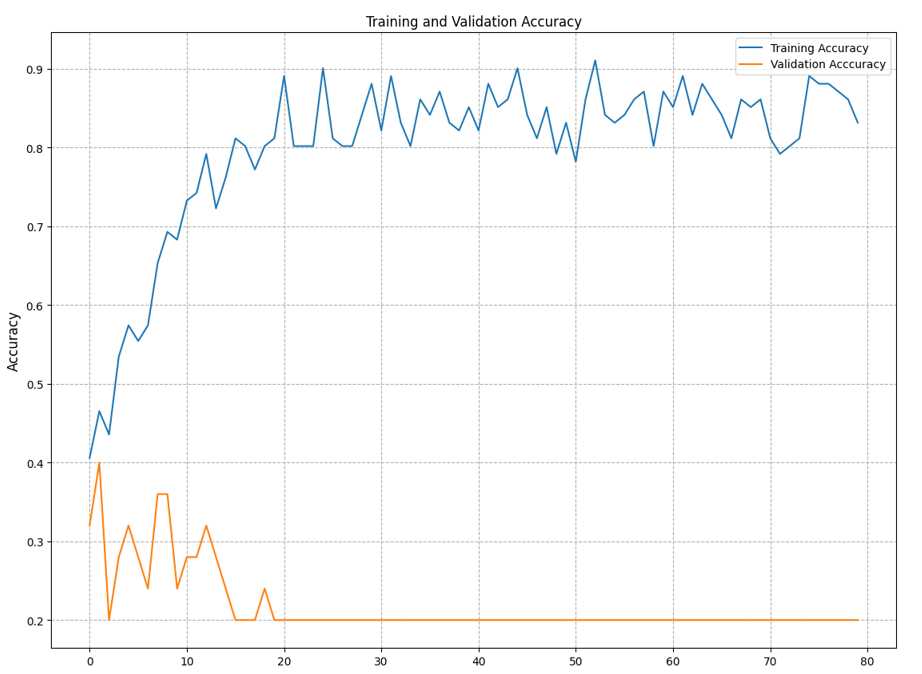
\includegraphics[scale=0.6]{gambar/AccIndRNNnoAug.png}
  % Keterangan gambar yang diinputkan
  \caption{Akurasi IndRNN Tanpa Data Augmentasi}
  % Label referensi dari gambar yang diinputkan
  \label{fig:AccIndRNNnoaug}
\end{figure}

\begin{figure} [H] \centering
  % Nama dari file gambar yang diinputkan
  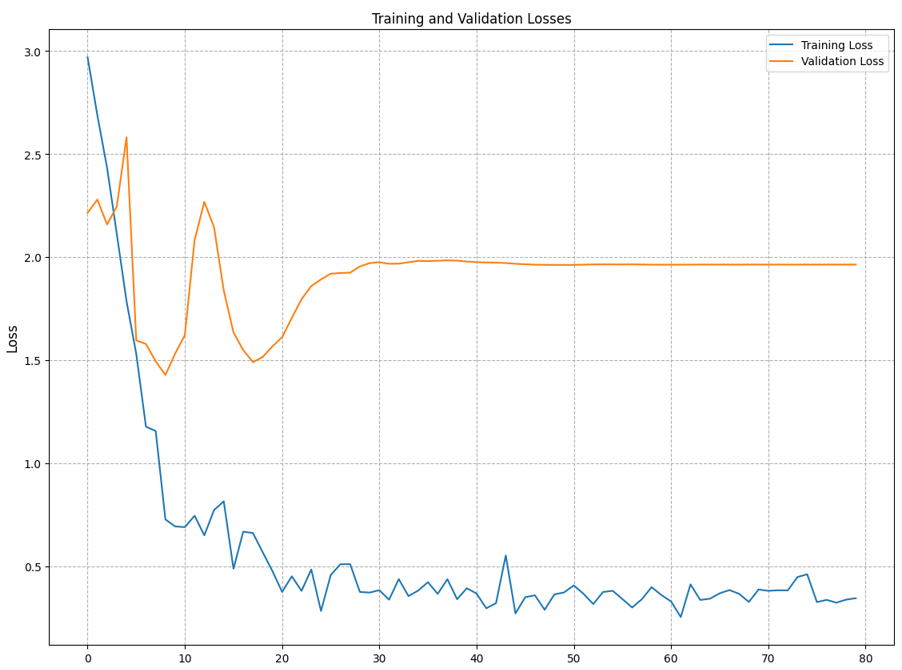
\includegraphics[scale=0.6]{gambar/LossIndRNNnoAug.png}
  % Keterangan gambar yang diinputkan
  \caption{Loss IndRNN Tanpa Data Augmentasi}
  % Label referensi dari gambar yang diinputkan
  \label{fig:LossIndRNNnoaug}
\end{figure}

\newpage
Berikut merupakan gambar loss dan akurasi dari data training yang teraugmentasi dan
data validasi yang terbaik:
\begin{figure} [H] \centering
  % Nama dari file gambar yang diinputkan
  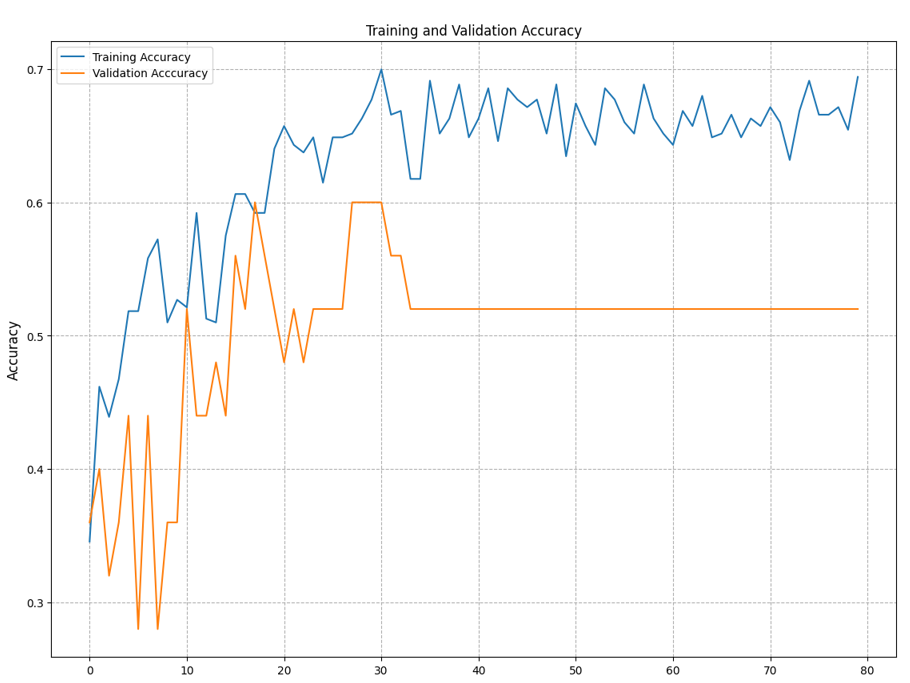
\includegraphics[scale=0.6]{gambar/AccIndRNNAug.png}
  % Keterangan gambar yang diinputkan
  \caption{Akurasi dan Loss IndRNN Dengan Data Augmentasi}
  % Label referensi dari gambar yang diinputkan
  \label{fig:AccIndRNNaug}
\end{figure}

\begin{figure} [H] \centering
  % Nama dari file gambar yang diinputkan
  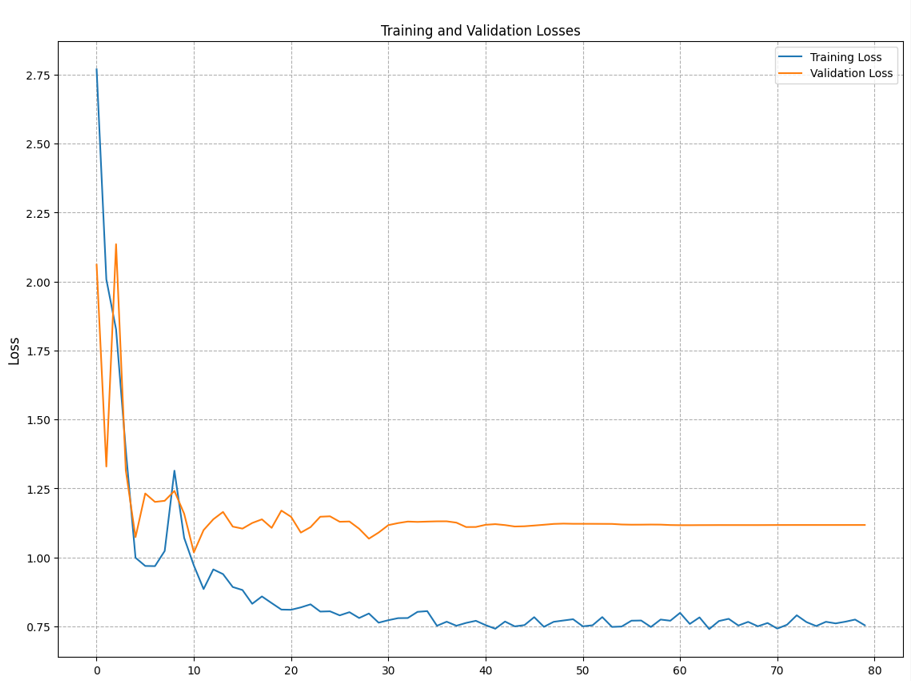
\includegraphics[scale=0.6]{gambar/LossIndRNNAug.png}
  % Keterangan gambar yang diinputkan
  \caption{Akurasi dan Loss IndRNN Dengan Data Augmentasi}
  % Label referensi dari gambar yang diinputkan
  \label{fig:LossIndRNNaug}
\end{figure}

Data pada gambar \ref{fig:AccIndRNNnoaug} dan gambar \ref{fig:LossIndRNNnoaug} menunjukkan akurasi training
sebesar 0.8378 dan akurasi validasi sebesar 0.2 serta loss training sebesar 0.3236
dan loss validasi sebesar 1.9798 . Sedangkan data pada gambar \ref{fig:AccIndRNNaug} dan gambar \ref{fig:LossIndRNNaug}
menunjukkan akurasi training sebesar 0.6943 dan akurasi validasi sebesar 0.52 serta
loss training sebesar 0.7529 dan loss validasi sebesar 1.1258 .

\subsection{Long short term memory network}
Berikut merupakan gambar loss dan akurasi dari data training yang tidak teraugmentasi dan
data validasi yang terbaik:

\begin{figure} [H] \centering
  % Nama dari file gambar yang diinputkan
  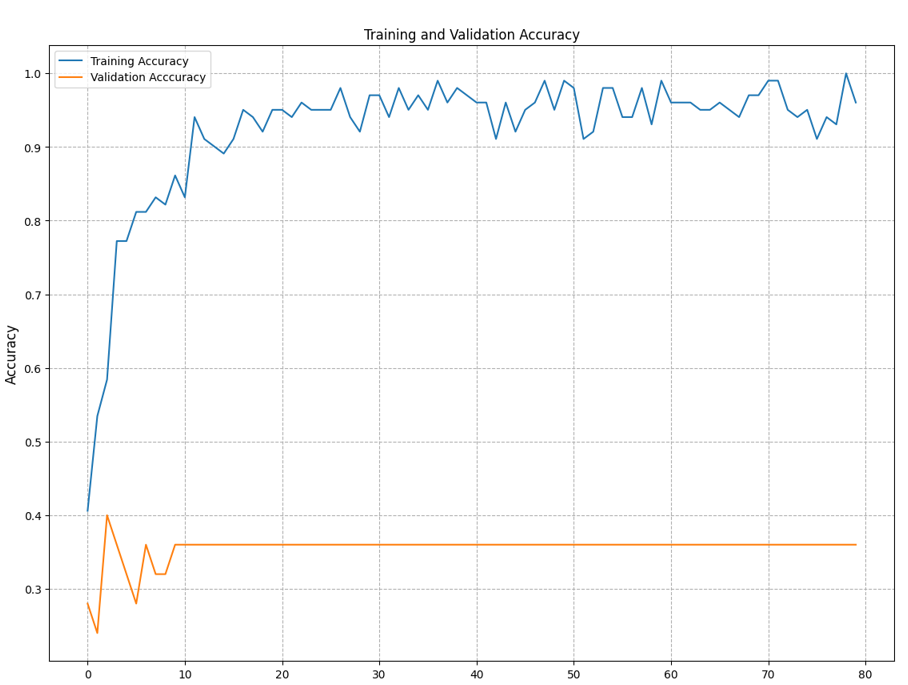
\includegraphics[scale=0.6]{gambar/AccLSTMnoAug.png}
  % Keterangan gambar yang diinputkan
  \caption{Akurasi dan Loss LSTM Tanpa Data Augmentasi}
  % Label referensi dari gambar yang diinputkan
  \label{fig:AccLSTMnoaug}
\end{figure}

\begin{figure} [H] \centering
  % Nama dari file gambar yang diinputkan
  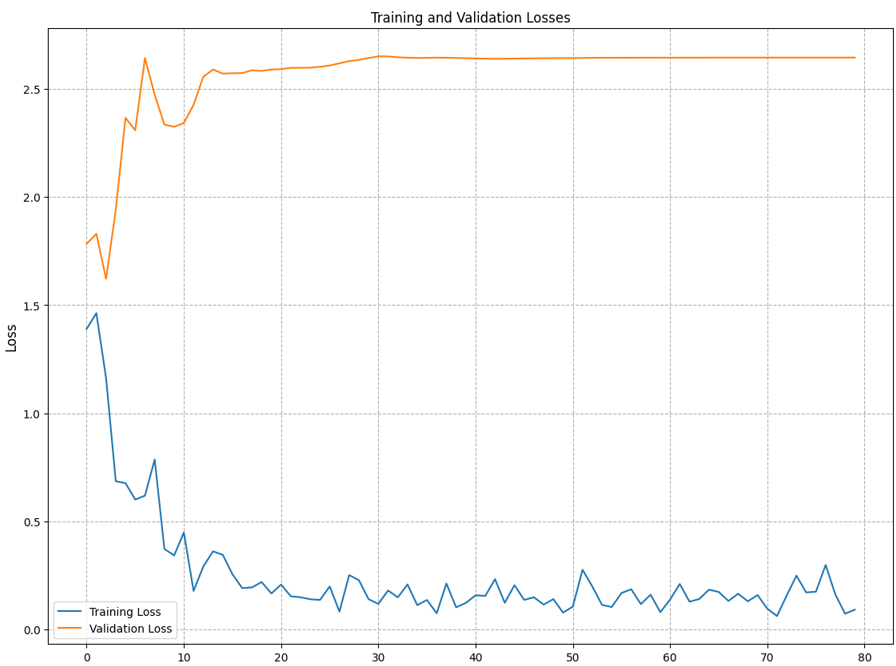
\includegraphics[scale=0.6]{gambar/LossLSTMnoAug.png}
  % Keterangan gambar yang diinputkan
  \caption{Akurasi dan Loss LSTM Tanpa Data Augmentasi}
  % Label referensi dari gambar yang diinputkan
  \label{fig:LossLSTMnoaug}
\end{figure}

\newpage
Berikut merupakan gambar loss dan akurasi dari data training yang teraugmentasi dan
data validasi yang terbaik:
\begin{figure} [H] \centering
  % Nama dari file gambar yang diinputkan
  \includegraphics[scale=0.6]{gambar/AccLSTMaug.png}
  % Keterangan gambar yang diinputkan
  \caption{Akurasi dan Loss LSTM Dengan Data Augmentasi}
  % Label referensi dari gambar yang diinputkan
  \label{fig:AccLSTMaug}
\end{figure}

\begin{figure} [H] \centering
  % Nama dari file gambar yang diinputkan
  \includegraphics[scale=0.6]{gambar/LossLSTMaug.png}
  % Keterangan gambar yang diinputkan
  \caption{Akurasi dan Loss LSTM Dengan Data Augmentasi}
  % Label referensi dari gambar yang diinputkan
  \label{fig:LossLSTMaug}
\end{figure}

Data pada gambar \ref{fig:AccLSTMnoaug} dan gambar \ref{fig:LossLSTMnoaug} menunjukkan akurasi training sebesar 0.9732
dan akurasi validasi sebesar 0.32 serta loss training sebesar 0.1342 dan loss validasi
sebesar 2.4947 . Sedangkan data pada gambar \ref{fig:AccLSTMaug} dan gambar \ref{fig:LossLSTMaug}
menunjukkan akurasi training sebesar 0.9354 dan akurasi validasi sebesar 0.4
serta loss training sebesar 0.3541 dan loss validasi sebesar 1.7487 .

\section{Hasil Evaluasi Model}
Hasil evaluasi yang dihasilkan pada penelitian ini berbentuk:
\begin{enumerate}[nolistsep]
  \item Confusion Matrix

        Confusion matrix adalah tabel yang menunjukkan jumlah prediksi yang benar dan salah yang dilakukan oleh
        model. Confusion matrix terdiri dari empat komponen: \emph{true positive} (TP), \emph{true negative} (TN), \emph{false
        positive} (FP), dan \emph{false negative} (FN). Dengan menggunakan confusion matrix, kita dapat menghitung
        metrik evaluasi lainnya.

  \item Akurasi

        Akurasi mengukur persentase prediksi yang benar secara keseluruhan. Ini dihitung dengan membagi jumlah
        prediksi yang benar (TP dan TN) dengan total sampel dalam dataset. Akurasi dapat memberikan gambaran
        umum tentang sejauh mana model dapat memprediksi dengan benar, tetapi dapat menghasilkan hasil yang
        bias jika terdapat ketimpangan jumlah sampel pada setiap kelas

  \item Presisi

        Presisi mengukur persentase prediksi positif yang benar. Ini mengukur sejauh mana prediksi positif
        model adalah akurat. Presisi dihitung dengan membagi TP dengan jumlah prediksi positif (TP dan FP).

  \item Recall

        Recall, juga dikenal sebagai \emph{Sensitivity} atau \emph{True Positive Rate} (TPR), mengukur persentase sampel
        positif yang diprediksi dengan benar. Ini mengukur sejauh mana model dapat menemukan semua sampel
        positif yang sebenarnya. Recall dihitung dengan membagi TP dengan jumlah sampel positif (TP dan FN).

  \item F1-Score

        F1-Score adalah penggabungan presisi dan recall menjadi satu metrik yang mencerminkan keseimbangan
        antara keduanya. F1-Score dihitung sebagai rata-rata harmonis dari presisi dan recall, dan memberikan
        gambaran keseluruhan tentang performa model. F1-Score berguna ketika kelas target memiliki
        ketidakseimbangan jumlah sampel.

\end{enumerate}

\subsection{Independent Recurrent Neural Network}

Berikut merupakan gambar hasil evaluasi model IndRNN tanpa data augmentasi:
\newpage
\begin{figure} [H] \centering
  % Nama dari file gambar yang diinputkan
  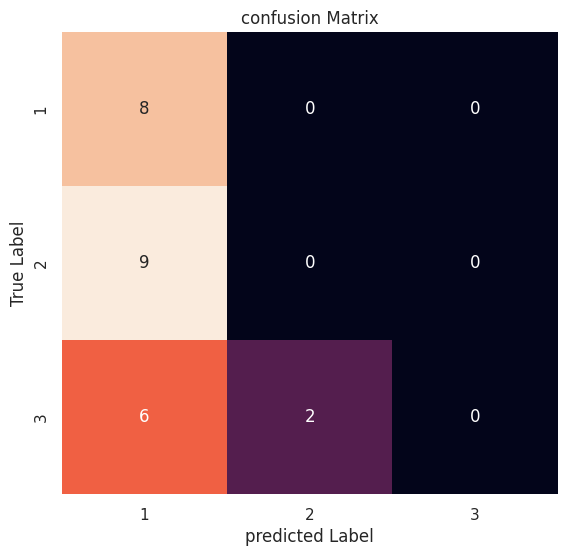
\includegraphics[scale=0.8]{gambar/CMIndRNNnoaug.png}
  % Keterangan gambar yang diinputkan
  \caption{Confusion Matrix IndRNN Tanpa Data Augmentasi}
  % Label referensi dari gambar yang diinputkan
  \label{fig:CMIndRNNnoaug}
\end{figure}

\begin{figure} [H] \centering
  % Nama dari file gambar yang diinputkan
  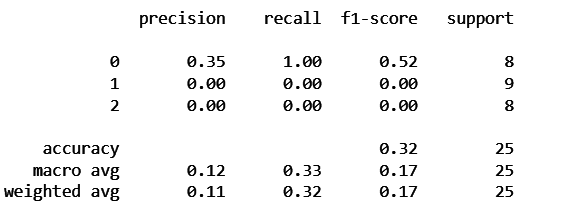
\includegraphics[scale=0.95]{gambar/scoreIndRNNnoaug.png}
  % Keterangan gambar yang diinputkan
  \caption{Evaluasi IndRNN Tanpa Data Augmentasi}
  % Label referensi dari gambar yang diinputkan
  \label{fig:ScoreIndRNNnoaug}
\end{figure}

Data yang didapatkan dari confusion matrix \ref{fig:CMIndRNNnoaug} didapatkan 8 video yang bernilai benar
dengan hasil akurasi sebesar 0.32, hasil nilai presisi model pada kelas 1 sebesar 0.35, hasil nilai
presisi model pada kelas 2 sebesar 0.0, hasil nilai presisi model pada kelas 3 sebesar 0.0. Model menghasilkan
nilai recall sebesar 1.0 pada kelas 1, 0.0 pada kelas 2, dan 0.0 pada kelas 3. Nilai f1-score yang dihasilkan
oleh model sebesar 0.52 pada kelas 1, 0.0 pada kelas 2, 0.0 pada kelas 3.

Berikut merupakan gambar hasil evaluasi model IndRNN  dengan data augmentasi:
\newpage
\begin{figure} [H] \centering
  % Nama dari file gambar yang diinputkan
  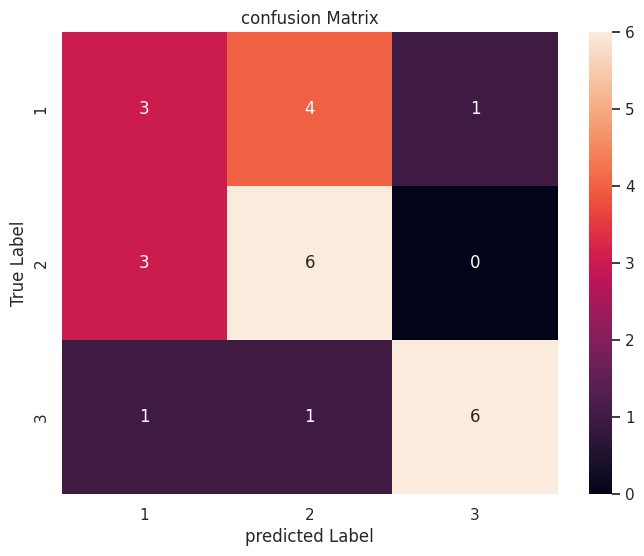
\includegraphics[scale=0.5]{gambar/CMIndRNNaug.png}
  % Keterangan gambar yang diinputkan
  \caption{Confusion Matrix IndRNN Dengan Data Augmentasi}
  % Label referensi dari gambar yang diinputkan
  \label{fig:CMIndRNNaug}
\end{figure}

\begin{figure} [H] \centering
  % Nama dari file gambar yang diinputkan
  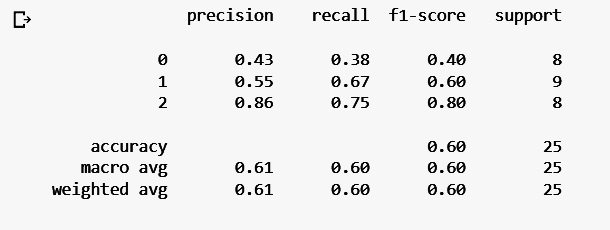
\includegraphics[scale=0.85]{gambar/scoreIndRNNaug.png}
  % Keterangan gambar yang diinputkan
  \caption{Evaluasi IndRNN Dengan Data Augmentasi}
  % Label referensi dari gambar yang diinputkan
  \label{fig:ScoreIndRNNaug}
\end{figure}

Data yang didapatkan dari confusion matrix \ref{fig:CMIndRNNaug} didapatkan 15 video yang bernilai benar
dengan hasil akurasi sebesar 0.6, hasil nilai presisi model pada kelas 1 sebesar 0.43, hasil nilai
presisi model pada kelas 2 sebesar 0.55, hasil nilai presisi model pada kelas 3 sebesar 0.86. Model menghasilkan
nilai recall sebesar 0.38 pada kelas 1, 0.67 pada kelas 2, dan 0.75 pada kelas 3. Nilai f1-score yang dihasilkan
oleh model sebesar 0.40 pada kelas 1, 0.60 pada kelas 2, 0.80 pada kelas 3.

\subsection{Long short term memory network}

Berikut merupakan gambar hasil evaluasi model LSTM tanpa data augmentasi:
\newpage
\begin{figure} [H] \centering
  % Nama dari file gambar yang diinputkan
  \includegraphics[scale=0.7]{gambar/CMLSTMnoAug.png}
  % Keterangan gambar yang diinputkan
  \caption{Akurasi dan Loss LSTM Tanpa Data Augmentasi}
  % Label referensi dari gambar yang diinputkan
  \label{fig:CMLSTMnoaug}
\end{figure}

\begin{figure} [H] \centering
  % Nama dari file gambar yang diinputkan
  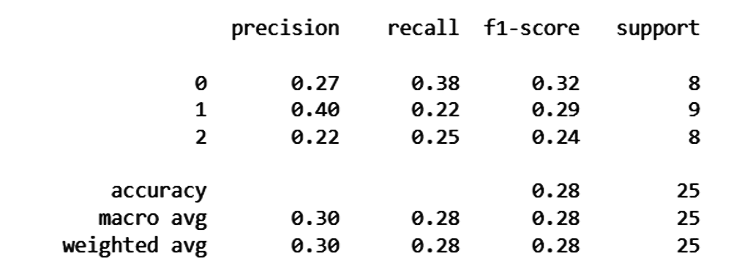
\includegraphics[scale=0.85]{gambar/scoreLSTMnoaug.png}
  % Keterangan gambar yang diinputkan
  \caption{Evaluasi LSTM Dengan Data Augmentasi}
  % Label referensi dari gambar yang diinputkan
  \label{fig:ScoreLSTMnoaug}
\end{figure}
Data yang didapatkan dari confusion matrix \ref{fig:CMLSTMnoaug} didapatkan 7 video yang bernilai benar
dengan hasil akurasi sebesar 0.28, hasil nilai presisi model pada kelas 1 sebesar 0.27, hasil nilai
presisi model pada kelas 2 sebesar 0.4, hasil nilai presisi model pada kelas 3 sebesar 0.22. Model menghasilkan
nilai recall sebesar 0.38 pada kelas 1, 0.22 pada kelas 2, dan 0.25 pada kelas 3. Nilai f1-score yang dihasilkan
oleh model sebesar 0.32 pada kelas 1, 0.29 pada kelas 2, 0.24 pada kelas 3.

Berikut merupakan gambar hasil evaluasi model LSTM dengan data augmentasi:
\begin{figure} [H] \centering
  % Nama dari file gambar yang diinputkan
  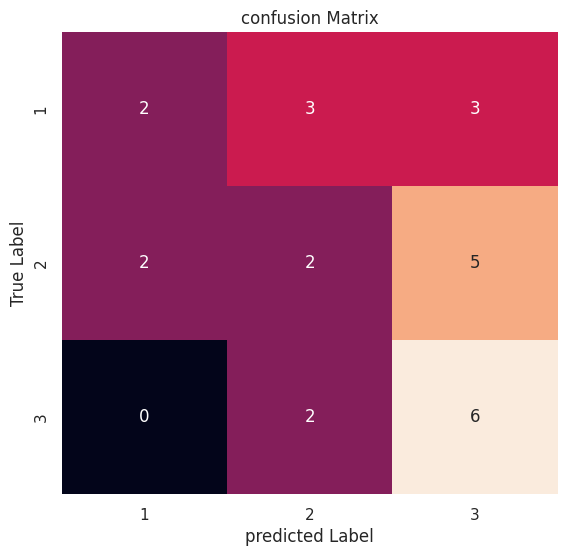
\includegraphics[scale=0.45]{gambar/CMLSTMaug.png}
  % Keterangan gambar yang diinputkan
  \caption{Confusion Matrix LSTM Dengan Data Augmentasi}
  % Label referensi dari gambar yang diinputkan
  \label{fig:CMLSTMaug}
\end{figure}

\begin{figure} [H] \centering
  % Nama dari file gambar yang diinputkan
  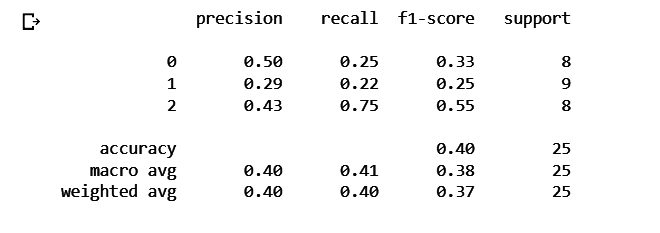
\includegraphics[scale=0.75]{gambar/scoreLSTMaug.png}
  % Keterangan gambar yang diinputkan
  \caption{Evaluasi LSTM Dengan Data Augmentasi}
  % Label referensi dari gambar yang diinputkan
  \label{fig:ScoreLSTMaug}
\end{figure}
Data yang didapatkan dari confusion matrix \ref{fig:CMLSTMaug} didapatkan 10 video yang bernilai benar
dengan hasil akurasi sebesar 0.40, hasil nilai presisi model pada kelas 1 sebesar 0.5, hasil nilai
presisi model pada kelas 2 sebesar 0.29, hasil nilai presisi model pada kelas 3 sebesar 0.43. Model menghasilkan
nilai recall sebesar 0.25 pada kelas 1, 0.22 pada kelas 2, dan 0.275 pada kelas 3. Nilai f1-score yang dihasilkan
oleh model sebesar 0.33 pada kelas 1, 0.25 pada kelas 2, 0.55 pada kelas 3.

\subsection{Support Vector Machine}
Berikut merupakan gambar hasil evaluasi model SVM tanpa data augmentasi:

\newpage
\begin{figure} [H] \centering
  % Nama dari file gambar yang diinputkan
  \includegraphics[scale=5]{gambar/CMSVMnoAug.png}
  % Keterangan gambar yang diinputkan
  \caption{Akurasi dan Loss SVM Tanpa Data Augmentasi}
  % Label referensi dari gambar yang diinputkan
  \label{fig:CMSVMnoaug}
\end{figure}

\begin{figure} [H] \centering
  % Nama dari file gambar yang diinputkan
  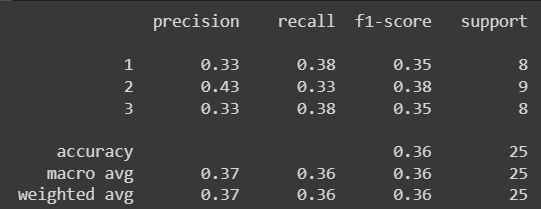
\includegraphics[scale=1]{gambar/scoreSVMnoaug.png}
  % Keterangan gambar yang diinputkan
  \caption{Evaluasi SVM Dengan Data Augmentasi}
  % Label referensi dari gambar yang diinputkan
  \label{fig:ScoreSVMnoaug}
\end{figure}

Data yang didapatkan dari confusion matrix 4.17 didapatkan 9 video yang bernilai benar
dengan hasil akurasi sebesar 0.36, hasil nilai presisi model pada kelas 1 sebesar 0.33, hasil
nilai presisi model pada kelas 2 sebesar 0.43, hasil nilai presisi model pada kelas 3 sebesar 0.33.
Model menghasilkan nilai recall sebesar 0.38 pada kelas 1, 0.33 pada kelas 2, dan 0.38 pada
kelas 3. Nilai f1-score yang dihasilkan oleh model sebesar 0.35 pada kelas 1, 0.38 pada kelas
2, 0.35 pada kelas 3.

Berikut merupakan gambar hasil evaluasi model SVM dengan data augmentasi:

\begin{figure} [H] \centering
  % Nama dari file gambar yang diinputkan
  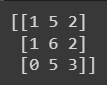
\includegraphics[scale=5]{gambar/CMSVMaug.png}
  % Keterangan gambar yang diinputkan
  \caption{Confusion Matrix SVM Dengan Data Augmentasi}
  % Label referensi dari gambar yang diinputkan
  \label{fig:CMSVMaug}
\end{figure}

\begin{figure} [H] \centering
  % Nama dari file gambar yang diinputkan
  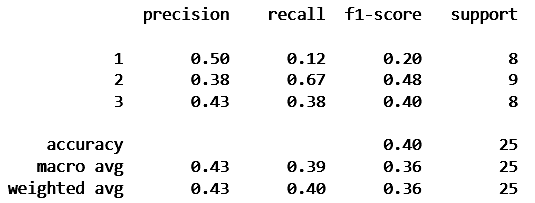
\includegraphics[scale=1]{gambar/scoreSVMaug.png}
  % Keterangan gambar yang diinputkan
  \caption{Evaluasi SVM Dengan Data Augmentasi}
  % Label referensi dari gambar yang diinputkan
  \label{fig:ScoreSVMaug}
\end{figure}

Data yang didapatkan dari confusion matrix 4.19 didapatkan 10 video yang bernilai benar
dengan hasil akurasi sebesar 0.40, hasil nilai presisi model pada kelas 1 sebesar 0.50, hasil
nilai presisi model pada kelas 2 sebesar 0.38, hasil nilai presisi model pada kelas 3 sebesar 0.43.
Model menghasilkan nilai recall sebesar 0.12 pada kelas 1, 0.67 pada kelas 2, dan 0.38 pada
kelas 3. Nilai f1-score yang dihasilkan oleh model sebesar 0.20 pada kelas 1, 0.48 pada kelas
2, 0.40 pada kelas 3.

\section{Hasil Testing Model}
\subsection{Independent Recurrent Neural Network}

Berikut merupakan gambar hasil evaluasi model IndRNN tanpa data augmentasi:
\newpage
\begin{figure} [H] \centering
  % Nama dari file gambar yang diinputkan
  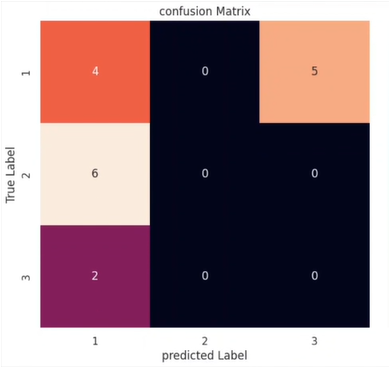
\includegraphics[scale=1.3]{gambar/CMIndRNNnoaug2.png}
  % Keterangan gambar yang diinputkan
  \caption{Confusion Matrix IndRNN Tanpa Data Augmentasi}
  % Label referensi dari gambar yang diinputkan
  \label{fig:CMIndRNNnoaug2}
\end{figure}

\begin{figure} [H] \centering
  % Nama dari file gambar yang diinputkan
  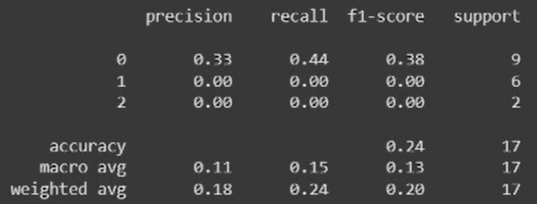
\includegraphics[scale=1]{gambar/scoreIndRNNnoaug2.png}
  % Keterangan gambar yang diinputkan
  \caption{Testing IndRNN Tanpa Data Augmentasi}
  % Label referensi dari gambar yang diinputkan
  \label{fig:ScoreIndRNNnoaug2}
\end{figure}

Data yang didapatkan dari confusion matrix \ref{fig:CMIndRNNnoaug2} didapatkan 4 video yang bernilai benar
dengan hasil akurasi sebesar 0.24, hasil nilai presisi model pada kelas 1 sebesar 0.33, hasil nilai
presisi model pada kelas 2 sebesar 0.0, hasil nilai presisi model pada kelas 3 sebesar 0.0. Model menghasilkan
nilai recall sebesar 0.44 pada kelas 1, 0.0 pada kelas 2, dan 0.0 pada kelas 3. Nilai f1-score yang dihasilkan
oleh model sebesar 0.38 pada kelas 1, 0.0 pada kelas 2, 0.0 pada kelas 3.

Berikut merupakan gambar hasil evaluasi model IndRNN  dengan data augmentasi:
\newpage
\begin{figure} [H] \centering
  % Nama dari file gambar yang diinputkan
  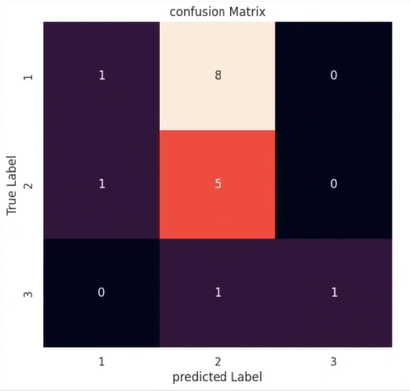
\includegraphics[scale=1.3]{gambar/CMIndRNNaug2.png}
  % Keterangan gambar yang diinputkan
  \caption{Confusion Matrix IndRNN Dengan Data Augmentasi}
  % Label referensi dari gambar yang diinputkan
  \label{fig:CMIndRNNaug2}
\end{figure}

\begin{figure} [H] \centering
  % Nama dari file gambar yang diinputkan
  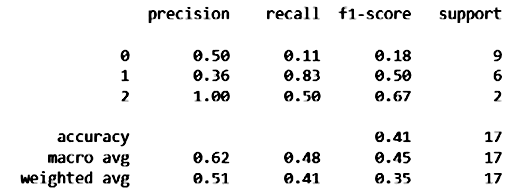
\includegraphics[scale=1]{gambar/scoreIndRNNaug2.png}
  % Keterangan gambar yang diinputkan
  \caption{Testing IndRNN Dengan Data Augmentasi}
  % Label referensi dari gambar yang diinputkan
  \label{fig:ScoreIndRNNaug}
\end{figure}

Data yang didapatkan dari confusion matrix \ref{fig:CMIndRNNaug2} didapatkan 7 video yang bernilai benar
dengan hasil akurasi sebesar 0.41, hasil nilai presisi model pada kelas 1 sebesar 0.50, hasil nilai
presisi model pada kelas 2 sebesar 0.36, hasil nilai presisi model pada kelas 3 sebesar 1.0. Model menghasilkan
nilai recall sebesar 0.11 pada kelas 1, 0.83 pada kelas 2, dan 0.50 pada kelas 3. Nilai f1-score yang dihasilkan
oleh model sebesar 0.18 pada kelas 1, 0.50 pada kelas 2, 0.67 pada kelas 3.

\subsection{Long short term memory network}

Berikut merupakan gambar hasil evaluasi model LSTM tanpa data augmentasi:
\newpage
\begin{figure} [H] \centering
  % Nama dari file gambar yang diinputkan
  \includegraphics[scale=1.3]{gambar/CMLSTMnoAug2.png}
  % Keterangan gambar yang diinputkan
  \caption{Akurasi dan Loss LSTM Tanpa Data Augmentasi}
  % Label referensi dari gambar yang diinputkan
  \label{fig:CMLSTMnoaug2}
\end{figure}

\begin{figure} [H] \centering
  % Nama dari file gambar yang diinputkan
  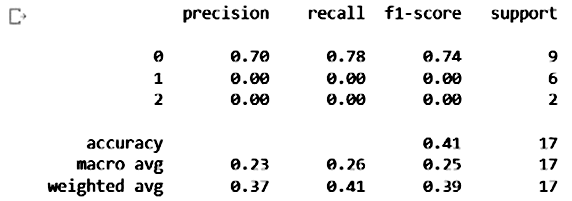
\includegraphics[scale=1]{gambar/scoreLSTMnoaug2.png}
  % Keterangan gambar yang diinputkan
  \caption{Testing LSTM Dengan Data Augmentasi}
  % Label referensi dari gambar yang diinputkan
  \label{fig:ScoreLSTMnoaug2}
\end{figure}
Data yang didapatkan dari confusion matrix \ref{fig:CMLSTMnoaug2} didapatkan 7 video yang bernilai benar
dengan hasil akurasi sebesar 0.41, hasil nilai presisi model pada kelas 1 sebesar 0.70, hasil nilai
presisi model pada kelas 2 sebesar 0.0, hasil nilai presisi model pada kelas 3 sebesar 0.0. Model menghasilkan
nilai recall sebesar 0.78 pada kelas 1, 0.0 pada kelas 2, dan 0.0 pada kelas 3. Nilai f1-score yang dihasilkan
oleh model sebesar 0.74 pada kelas 1, 0.0 pada kelas 2, 0.0 pada kelas 3.

Berikut merupakan gambar hasil evaluasi model LSTM dengan data augmentasi:
\begin{figure} [H] \centering
  % Nama dari file gambar yang diinputkan
  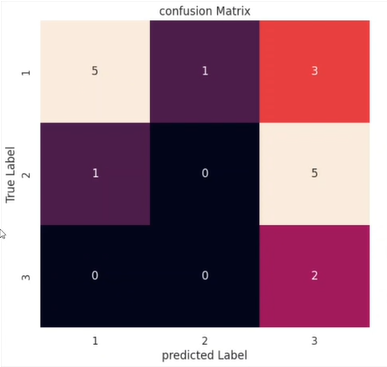
\includegraphics[scale=1.3]{gambar/CMLSTMaug2.png}
  % Keterangan gambar yang diinputkan
  \caption{Confusion Matrix LSTM Dengan Data Augmentasi}
  % Label referensi dari gambar yang diinputkan
  \label{fig:CMLSTMaug2}
\end{figure}

\begin{figure} [H] \centering
  % Nama dari file gambar yang diinputkan
  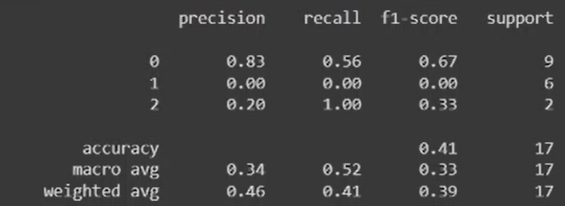
\includegraphics[scale=1]{gambar/scoreLSTMaug2.png}
  % Keterangan gambar yang diinputkan
  \caption{Testing LSTM Dengan Data Augmentasi}
  % Label referensi dari gambar yang diinputkan
  \label{fig:ScoreLSTMaug2}
\end{figure}
Data yang didapatkan dari confusion matrix \ref{fig:CMLSTMaug2} didapatkan 7 video yang bernilai benar
dengan hasil akurasi sebesar 0.41, hasil nilai presisi model pada kelas 1 sebesar 0.83, hasil nilai
presisi model pada kelas 2 sebesar 0.0, hasil nilai presisi model pada kelas 3 sebesar 0.20. Model menghasilkan
nilai recall sebesar 0.56 pada kelas 1, 0.0 pada kelas 2, dan 1.0 pada kelas 3. Nilai f1-score yang dihasilkan
oleh model sebesar 0.67 pada kelas 1, 0.0 pada kelas 2, 0.33 pada kelas 3.

\subsection{Support Vector Machine}
Berikut merupakan gambar hasil evaluasi model SVM tanpa data augmentasi:

\newpage
\begin{figure} [H] \centering
  % Nama dari file gambar yang diinputkan
  \includegraphics[scale=5]{gambar/CMSVMnoAug2.png}
  % Keterangan gambar yang diinputkan
  \caption{Akurasi dan Loss SVM Tanpa Data Augmentasi}
  % Label referensi dari gambar yang diinputkan
  \label{fig:CMSVMnoaug2}
\end{figure}

\begin{figure} [H] \centering
  % Nama dari file gambar yang diinputkan
  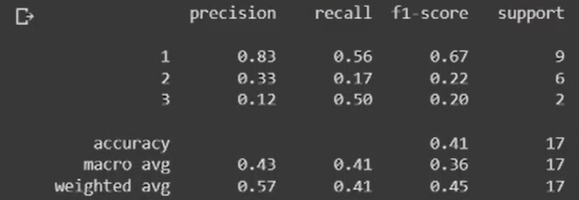
\includegraphics[scale=1]{gambar/scoreSVMnoaug2.png}
  % Keterangan gambar yang diinputkan
  \caption{Testing SVM Dengan Data Augmentasi}
  % Label referensi dari gambar yang diinputkan
  \label{fig:ScoreSVMnoaug2}
\end{figure}

Data yang didapatkan dari confusion matrix \ref{fig:CMSVMnoaug2} didapatkan 7 video yang bernilai benar
dengan hasil akurasi sebesar 0.41, hasil nilai presisi model pada kelas 1 sebesar 0.83, hasil
nilai presisi model pada kelas 2 sebesar 0.33, hasil nilai presisi model pada kelas 3 sebesar 0.12.
Model menghasilkan nilai recall sebesar 0.56 pada kelas 1, 0.17 pada kelas 2, dan 0.50 pada
kelas 3. Nilai f1-score yang dihasilkan oleh model sebesar 0.67 pada kelas 1, 0.22 pada kelas
2, 0.20 pada kelas 3.

Berikut merupakan gambar hasil evaluasi model SVM dengan data augmentasi:

\begin{figure} [H] \centering
  % Nama dari file gambar yang diinputkan
  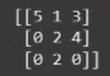
\includegraphics[scale=5]{gambar/CMSVMaug2.png}
  % Keterangan gambar yang diinputkan
  \caption{Confusion Matrix SVM Dengan Data Augmentasi}
  % Label referensi dari gambar yang diinputkan
  \label{fig:CMSVMaug2}
\end{figure}

\begin{figure} [H] \centering
  % Nama dari file gambar yang diinputkan
  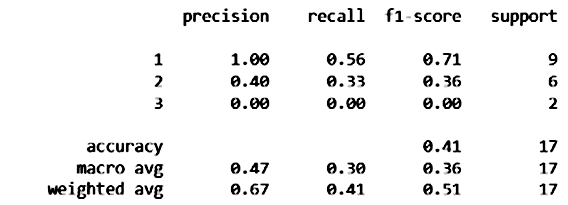
\includegraphics[scale=1]{gambar/scoreSVMaug2.png}
  % Keterangan gambar yang diinputkan
  \caption{Testing SVM Dengan Data Augmentasi}
  % Label referensi dari gambar yang diinputkan
  \label{fig:ScoreSVMaug2}
\end{figure}

Data yang didapatkan dari confusion matrix \ref{fig:CMSVMaug2} didapatkan 7 video yang bernilai benar
dengan hasil akurasi sebesar 0.41, hasil nilai presisi model pada kelas 1 sebesar 1.0, hasil
nilai presisi model pada kelas 2 sebesar 0.40, hasil nilai presisi model pada kelas 3 sebesar 0.0.
Model menghasilkan nilai recall sebesar 0.56 pada kelas 1, 0.33 pada kelas 2, dan 0.0 pada
kelas 3. Nilai f1-score yang dihasilkan oleh model sebesar 0.71 pada kelas 1, 0.36 pada kelas
2, 0.0 pada kelas 3.

\newpage
\section{Pembahasan}
\label{sec:analisispengujian}

Dari pengujian yang telah dilakukan, berdasarkan hasil training kedua model
yaitu dengan IndRNN dan LSTM didapatkan tabel sebagai berikut:

% Contoh pembuatan tabel
\begin{longtable}{|c|c|c|c|c|}
  \caption{Data Hasil Training Model}
  \label{tb:EnergiKecepatan}                                                                                            \\
  \hline
  \rowcolor[HTML]{C0C0C0}
  \textbf{Model}                & \textbf{Akurasi} & \textbf{Validasi} & \textbf{Loss Akurasi} & \textbf{Loss Validasi} \\
  \hline
  IndRNN tanpa data augmentasi  & 0.8378           & 0.2               & 0.3236                & 1.9798                 \\
  IndRNN dengan data augmentasi & 0.6943           & 0.52              & 0.7529                & 1.1258                 \\
  LSTM tanpa data augmentasi    & 0.9732           & 0.32              & 0.1342                & 2.4947                 \\
  LSTM dengan data augmentasi   & 0.9354           & 0.4               & 0.3541                & 1.7487                 \\
  \hline
\end{longtable}

\begin{longtable}{|c|c|}
  \caption{Data Hasil Evaluasi Model}
  \label{tb:EnergiKecepatan}                                \\
  \hline
  \rowcolor[HTML]{C0C0C0}
  \textbf{Model}                & \textbf{Confusion Matrix} \\
  \hline
  IndRNN tanpa data augmentasi  & 8 data benar              \\
  IndRNN dengan data augmentasi & 15 data benar             \\
  LSTM tanpa data augmentasi    & 7 data benar              \\
  LSTM dengan data augmentasi   & 10 data benar             \\
  SVM tanpa data augmentasi     & 9 data benar              \\
  SVM dengan data augmentasi    & 10 data benar             \\
  \hline
\end{longtable}

Model yang pertama yaitu IndRNN dengan input (x) berupa nilai EAR serta MAR dan kelas
sebagai target (y) mendapatkan hasil training yang kurang baik dengan akurasi sebesar 0.8378 dan validasi akurasi sebesar 0.2,
pada grafik terlihat model mengalami overfitting.

Model yang kedua yaitu IndRNN dengan input (x) berupa nilai EAR serta MAR yang teraugmentasi dan kelas
sebagai target (y) mendapatkan hasil training yang paling baik diantara model lainnya karena tidak mengalami
overfitting dengan akurasi 0.6943 dan validasi akurasi 0.52.

Model yang ketiga yaitu LSTM dengan input (x) berupa nilai EAR serta MAR dan kelas
sebagai target (y) mendapatkan hasil training yang kurang baik dengan akurasi sebesar 0.9732 dan validasi akurasi sebesar 0.32
, pada grafik terlihat model mengalami overfitting.

Model yang keempat yaitu LSTM dengan input (x) berupa nilai EAR serta MAR yang teraugmentasi dan kelas
sebagai target (y) mendapatkan hasil training yang lebih baik daripada LSTM dengan data yang tidak teraugmentasi,
selain itu pada grafik juga terlihat model mengalami overfitting dengan akurasi 0.9354 dan validasi akurasi 0.4.

Model yang kelima yaitu SVM dengan input (x) berupa nilai EAR serta MAR dan kelas
sebagai target (y) mendapatkan hasil evaluasi yang lebih baik jika dibandingkan dengan IndRNN dan LSTM tanpa data
augmentasi yang menghasilkan 10 nilai benar.

Model yang keenam yaitu SVM dengan input (x) berupa nilai EAR serta MAR yang teraugmentasi dan kelas
sebagai target (y) mendapatkan hasil evaluasi yang lebih baik daripada SVM dengan data yang tidak teraugmentasi.

Berdasarkan keseluruhan hasil training dan evaluasi, didapatkan bahwa model klasifikasi terbaik yaitu model IndRNN yang
ditraining menggunakan data yang telah diaugmentasi. Hal ini memvalidasi bahwa kinerja IndRNN pada klasifikasi kantuk
lebih baik daripada menggunakan SVM dan LSTM.
